\documentclass[12pt]{article}
\usepackage[utf8]{inputenc}
\usepackage[top=0.75in, bottom=0.75in, left=0.75in, right=0.75in, headheight=15pt]{geometry}
\usepackage{amsmath, amssymb, amsthm, graphicx, hyperref, enumerate, multirow,  multicol, tikz, centernot, cancel, forest, lipsum, mathtools, bm, esvect, fancyhdr, esdiff, float, parskip, comment}

\DeclareMathSymbol{*}{\mathbin}{symbols}{"01} % change * to /cdot inside math
% \begingroup % let only this align, etc. break across pages
% \allowdisplaybreaks
% \begin{align}
%     ....
% \end{align}
% \endgroup

% \begin{figure}[H]
%     \centering
%     \includegraphics{}
%     \caption{}
%     \label{fig:}
% \end{figure}

% \texorpdfstring{$k$}{k} math inside (sub/)section label

\pagestyle{fancy}
\fancyhead[L]{Liheng Cao}
% \fancyhead[C]{center}
\fancyhead[R]{}

\title{} % title
\author{Liheng Cao} % name
\date{\today} % custom date else today's date

\begin{document}
\maketitle

\section{}
\begin{enumerate}[(a)]
	\item \,\begin{figure}[H]
		\centering
		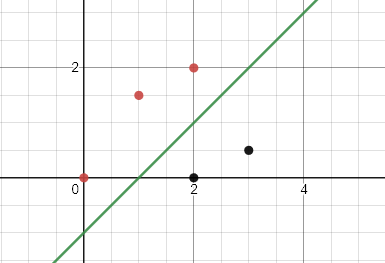
\includegraphics{images/1a.png}
		\caption{horizontal axis: $x_0$, vertical axis: $ x_1 $}
		\label{fig:1:a}
	\end{figure}

	\item They are linearly separable.
	
	\item
		\begin{enumerate}[i.]
			\item\,
			\begin{table}[H]
				\centering
					\begin{tabular}{|c|c|c|c|}
					\hline 
					$x_1$ & $ x_2 $ & $ y $ & functional margin\\\hline
					\hline
					0 & 0 & -1 & -3\\\hline
					2 & 2 & -1 & -3\\\hline
					2 & 0 & 1 & 3\\\hline
					1 & 1.5 & -1 & -4.5\\\hline
					3 & 0.5 & 1 & 4.5\\\hline				
				\end{tabular}
			\end{table}
			The absolute minimum is 3. 
		
			\item To find the geometric margin, we just divide everything by $ \|w\|_{2} = \sqrt{3^2 + 3^2}  = 3\sqrt{2}$.
			\begin{table}[H]
				\centering
				\begin{tabular}{|c|c|c|c|}
					\hline 
					$x_1$ & $ x_2 $ & $ y $ & geometric margin\\\hline
					\hline
					0 & 0 & -1 & $ -\frac{1}{\sqrt{2}} $\\\hline
					2 & 2 & -1 & $ -\frac{1}{\sqrt{2}} $\\\hline
					2 & 0 & -1 & $ \frac{1}{\sqrt{2}} $\\\hline
					1 & 1.5 & -1 & $ -\frac{3}{2\sqrt{2}} $\\\hline
					3 & 0.5 & 1 & $ \frac{3}{2\sqrt{2}} $\\\hline				
				\end{tabular}
			\end{table}
			The absolute minimum is $ \dfrac{1}{\sqrt{2}} $
			
			\item We divide $ w, w_0 $ by the functional margin to get the canonical weights. They are $ [3, -3]/3 = [1, -1], -3/3 = -1 $		
		\end{enumerate}
	
		\item The first 3 examples are support vectors because they have the same absolute margin (doesn't matter which type of margin since they are just a constant multiple of each other).
		
		\item $ (1,3)^T(1,-1) - 1 = 1 -3 -1 = -3 $. $ y(x^Tw_{canon} - w_{0, canon}) > 1 $ meaning it is on the correct side of the hyperplane and it is not a support vector. Since it's the value is greater than 1, the margin does not change.
		
		\item Without doing any calculations, neither of them change. It isn't a support vector to begin with and there are multiple support vectors, so removing one of them wouldn't change the margins. There is no risk of a data set begin no longer separable if we remove something; this risk is only present when we're adding something.
		
		\item Without doing any calculations, neither of them change. Even though this point is a support vector, it was not the only one, meaning that that the canonical margins would not change. Likewise, the separating plane would not change because there is no risk when removing a point.
		
		\item minimize $ w_0^2 + w_1^2 + w_2^2 $
		\par subject to :
		\begin{align*}
			-1 *(w_0 + 0 * w_1 + 0 * w_2) &\geq 1\\
			-1 *(w_0 + 2 * w_1 + 2 * w_2) &\geq 1\\
			1 *(w_0 + 2 * w_1 + 0 * w_2) &\geq 1\\
			-1 *(w_0 + 1 * w_1 + 1.5 * w_2) &\geq 1\\
			1 *(w_0 + 3 * w_1 + 0.5 * w_2) &\geq 1
		\end{align*}
\end{enumerate}
\newpage

\section{}
Yes. 
\par max $ \gamma $, subject to :
\begin{align*}
	y^{(i)}(w_0+\mathbf{w}^Tx^{(i)}) &\geq \gamma\\
	\|\mathbf{w}\|_{2} &= 1
\end{align*}

is equivalent to 
\par min $ \|\mathbf{w}\|_{2}^{2} $, subject to :
\begin{align*}
	y^{(i)}(w_0+\mathbf{w}^Tx^{(i)}) &\geq 1
\end{align*}
\par Both are trying to find the parameters that make the margin as large as possible. The first tries to maximize the margin directly, and keeps the magnitude of the parameters constant to prevent the ``constant multiple" trick. The second takes the opposite approach: it tries to minimize the parameters, while keeping margin a constant value.
\newpage

\section{}
\[ \xi^{(i)} =  \begin{cases}
	0 & y^{(i)}(\mathbf{w}^T\mathbf{x}^{(i)}) \geq 1\\
	1 - y^{(i)}(\mathbf{w}^T\mathbf{x}^{(i)}) & \text{otherwise}
\end{cases} \]
\begin{enumerate}[(a)]
	\item If $ \xi^{(i)} = 0$, the point is correctly classified and outside of the margin.
	
	\item If $ 0 < \xi^{(i)} < 1$, the point is correctly classified, but it is very close to the hyperplane and inside the margin.
	
	\item If $ \xi^{(i)} > 1 \rightarrow y^{(i)}(\mathbf{w}^T\mathbf{x}^{(i)}) < 0$, the point is incorrectly classified. 
\end{enumerate}
\newpage

\section{}

	
	
\end{document}